
\noindent \textbf{15. PC 111105} (Cortes de tora) Você deve cortar uma tora de madeira em vários pedaços. A empresa mais em conta para fazer isso é a \textit{Analog Cutting Machinery} (ACM), que cobra de acordo com o comprimento da tora a ser cortada. A máquina de corte deles permite que apenas um corte seja feito por vez. Se queremos fazer vários cortes, é fácil ver que ordens diferentes destes cortes levam a preços diferentes. Por exemplo, considere uma tora com 10 metros de comprimento, que tem que ser cortada a 2, 4 e 7 metros de uma de suas extremidades. Há várias possibilidades. Podemos
primeiramente fazer o corte dos 2 metros, depois dos 4 e depois dos 7. Tal ordem custa 10+8+6 = 24, porque a primeira tora tinha comprimento 10, o que restou tinha 8 metros de comprimento e o último pedaço tinha comprimento 6. Se cortássemos na ordem 4, depois 2, depois 7, pagaríamos 10 + 4 + 6 = 20, que é mais barato.\\
Seu chefe encomendou um programa que, dado o comprimento $l$ da tora e $k$ pontos $p_1,... , p_k$ de corte da tora, encontre o custo mínimo para executar esses cortes na ACM.

\textbf{Resposta:} Assumindo que os pontos de corte estão ordenados, ou seja, $p_1 \leq p_2 \leq p_3 \leq ... \leq p_n$, podemos olhar este problema de forma semelhante ao da ABB ótima.

Antes de mais nada, devemos inserir o valor $0$ na posição $0$ de $p$ e o tamanho $l$ da tora na posição $p_{k+1}$, para que possamos calcular o tamanho restante da tora após um corte.

Podemos. então, caracterizar a \textbf{suesbtrutura ótima} da seguinte maneira: se o custo de corte da tora $t$ de t$[i..j]$ é mínimo, então, o custo de corte da tora de $t[i..m]$ e $t[m..j]$ também é mínimo.

Vamos definir por $c[i, j]$ o custo mínimo de corte da tora de $t[i..j]$. Vejamos agora a \textbf{recorrência} para calcular o custo mínimo de corte da tora:

\begin{align*}
c[i, j] = \left\{\begin{array}{rl}
                    0, &\mbox{se $i + 1 = j$} \\
                    \smash{\displaystyle\min_{i < m < j}} {c[i, m] + c[m, j]} + p_j - p_i, &\mbox{se $i+1 < j $}
                \end{array} \right.
\end{align*}

A figura \ref{fig:6.15-1} mostra a tabela $c[i, j]$ preenchida após todas as iterações para a entrada $p = \langle 4, 5, 7, 8 \rangle$ e $l = 10$. A matriz será preenchida pelas diagonais, de cima para baixo. Vale lembrar que inserimos os valores 0 e $l$ em $p$ antes de executar a recorrência, resultando em $p' = \langle 0, 4, 5, 7, 8, 10 \rangle$.

\begin{center}
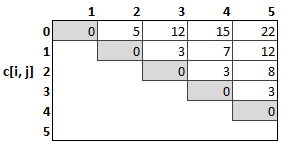
\includegraphics[width=0.45\textwidth]{q6-15-p1.png}
\captionof{figure}{Matriz $c$ preenchida após todas as iterações}
\label{fig:6.15-1}
\end{center}

O algorimto \proc{Analog-Cutting-Machinery} calcula o custo mínimo de corte da tora, com base na recorrência dada por $c[i, j]$.

\begin{codebox}
\Procname{$\proc{Analog-Cutting-Machinery}(p, l)$}
\li $\proc{Insert}(p, 0, 0)$
\li $\proc{Insert}(p, \attrib{p}{length}, l)$
\li $n \gets \attrib{p}{length}$
\li \For $i \gets 0$ \To $n-1$
\li \Do
        $c[i, i+1] \gets 0$
    \End
\li \For $k \gets 1$ \To $n$
\li \Do
        \For $i \gets 0$ \To $n - k - 1$
\li     \Do
            $j \gets i + k + 1$
\li         $c[i, j] \gets \infty$
\li         \For $m \gets i+1$ \To $j$
\li         \Do
                $aux \gets c[i, m] + c[m, j]$
\li             \If $aux < c[i, j]$
\li             \Then
                    $c[i, j] \gets aux$
                \End
            \End
\li         $c[i, j] = c[i, j] + p[j] - p[i]$
        \End 
    \End
\li \Return $c[0, n]$
\end{codebox}

O custo mínimo do corte da tora é retornado na posição $c[0, n]$. A tabela \ref{tbl:6-15-1} mostra o tempo de execução do algoritmo $\proc{Analog-Cutting-Machinery}$. Como as inserções em $p$ nas linhas 1-2 podem ser feitas em tempo $\Theta(n)$, o consumo total é $\Theta(n^3)$. já que as linhas 6-14 têm 3 \textit{loops} encadeados que tomam, no máximo, $n$ iterações cada um.

\begin{table}[H]
\centering
\begin{tabular}{|l|l|}
\hline
Linha                   & Tempo \\ \hline
1-2 & $\Theta(n)$ \\ \hline
3 & $\Theta(1)$ \\ \hline
4-5 & $\Theta(n)$ \\ \hline
6-14 & $\Theta(n^3)$ \\ \hline
15 & $\Theta(1)$ \\ \hline
Total & $\Theta(3n) + \Theta(n^3) = \Theta(n^3)$ \\ \hline
\end{tabular}
\caption{Tempo de execução}
\label{tbl:6-15-1}
\end{table}